\subsection{Le laboratoire et ses relations institutionnelles}
Le Laboratoire de l'Informatique du Parallélisme (abrégé \gls{lip}) est un laboratoire de recherche en informatique situé principalement sur le site Monod de l'École Normale Supérieure de Lyon.

\subsubsection{Présentation générale}
Créé dans les années 80, le Laboratoire de L'Informatique du Parallélisme devient \gls{ura} (URA) de l'\gls{ens} Lyon en 1989, puis \gls{umr} (UMR) en 1999 qui sera complété par l'Université Claude Bernard Lyon 1 en 2003. Le laboratoire est très tôt épaulé par l'Institut national de recherche en informatique et en automatique (\gls{inria}) qui est le principal acteur de la recherche en informatique et mathématique en France depuis 1967. Ainsi le laboratoire héberge plusieurs équipes-projets communes avec l'\gls{inria}. \cite{reportHCERES}\\

Le laboratoire compte 57 enseignant titulaires et chercheurs, entre 40 et 50 doctorants ainsi qu'une vingtaine de personnes sur des postes non permanents. L'équipe d'administration et l'équipe technique quant-à-elles sont épaulés par 12 ingénieurs.\\

Le \gls{lip} possède une bonne visibilité de ses équipes au niveau national et de plusieurs de ses membres au niveau international. Il occupe une place central dans le paysage de la recherche en informatique français pour quasiment l'ensemble de ses thématiques. La forte croissance du laboratoire lui a même obligé a s'étendre sur 2 autres sites : au sein de l’Institut Rhône-Alpin des Systèmes Complexes, et au sein de locaux appartenant à l’UCB à Gerland.

\subsubsection{Organisation générale}
Le laboratoire compose l'\gls{umr} 5668 avec l'ENS Lyon (EnsL), l'Université Claude Bernard Lyon 1, l'\gls{inria} et le CNRS. Il est dirigé par \textbf{M. Patrick Baillot} qui est secondé par \textbf{M. Frédéric Vivien}. Le responsable en charge de l'appel à projets, de la valorisation de recherche et des relations internationales est \textbf{M. Eddy Caron} et le responsable en charge des thèses, de l'enseignement et des postes non permanents est \textbf{M. Damien Stehlé}.

L'équipe administrative et l'équipe en charge des moyens informatique quant-à-elles sont composés de différentes personne issues des institutions qui constituent l'\gls{umr} 5668.\\

Le laboratoire héberge sept équipes de recherche dont cinq sont commune avec l'\gls{inria} : AriC, Avalon, CASH, DANTE, MC2, PLUME et ROMA chacune administrés par un chef d'équipe.

\begin{figure}[h]
	\center
	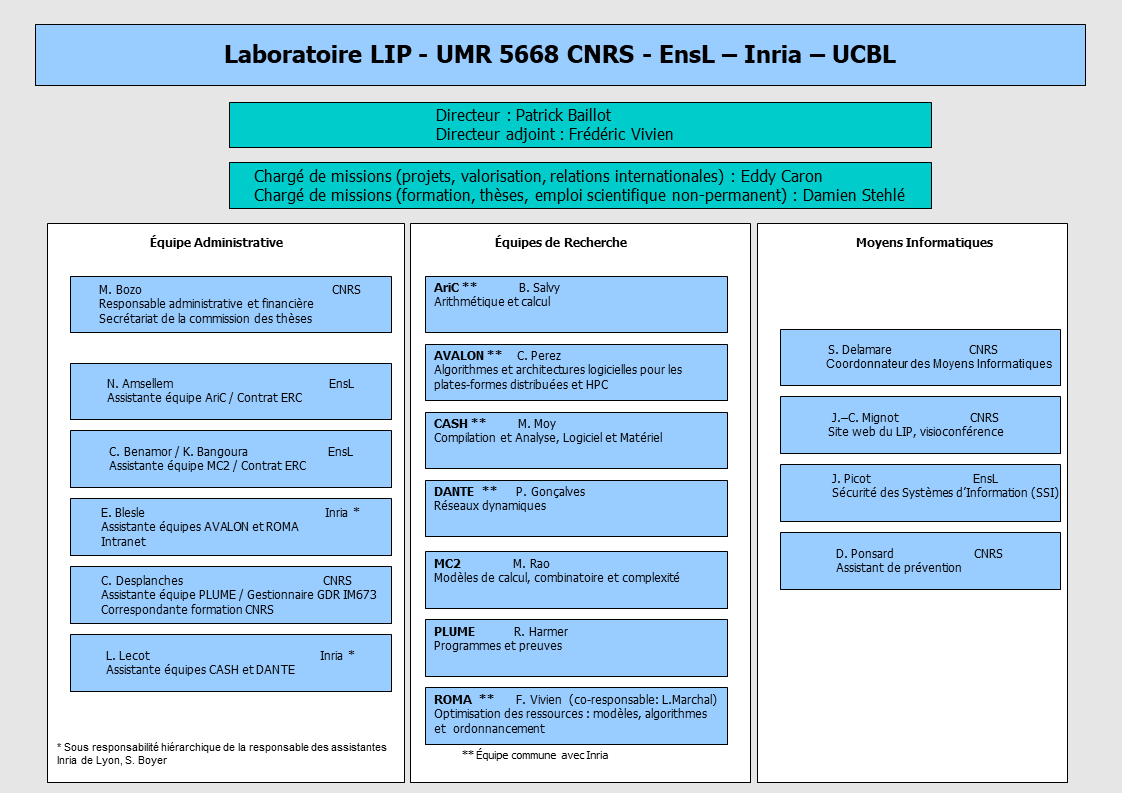
\includegraphics[scale=0.5]{partie1/images/organigramme.png}
	\caption{Organigramme du LIP au 10 Avril 2018 \cite{organigramme}}
\end{figure}
\subsubsection{Des métiers variés}
Le projet du Laboratoire de l'Informatique du Parallélisme est de mettre en relation l'informatique fondamental et sa mise en œuvre pratique dans les institutions. Ainsi le laboratoire crée un lien fort entre informatique et d'autres sciences comme les mathématiques, les sciences du vivant ou, plus globalement, les sciences fondamentales.\cite{presUCBL}\\

Les chercheurs du \gls{lip} possèdent un socle commun : l'algorithmie et l'utilisation efficace des ressources. Ils organisent leurs recherches autour de deux grands axes :
\begin{itemize}
	\item La conception, l'utilisation et l'adéquation aux besoins des applications des futurs architectures de calcul (traitement de données, calcul fondamental) et de communication (réseaux)
	\item L'étude des modèles et des méthodes en informatique : compléxité, algorithmie, développement logiciel et matériel, avancée technologiques etc.\\
\end{itemize}

Ainsi, le laboratoire ne compte pas dans ses rang uniquement des expert de l'informatique. D'autres profils bien différents sont mis en valeurs dans les 7 équipes-projets que nous allons présenter.
\newpage

\textbf{AriC - Arithmetic and Computing}\\
AriC est une grande équipe projet commune avec l'\gls{inria} composée d'une vingtaine de membres. Elle à pour but d'améliorer le calcul, en terme de performance, d'efficacité et de fiabilité. Ses 3 principaux projets de recherche portent sur les sujets suivants :
\begin{itemize}
	\item Les réseaux euclidiens : algorithme et cryptologie,
	\item Les méthodes d'approximation efficaces en calcul formel,
	\item Le calcul fiable à haute performance, avec virgule flottante et précision d'au plus une centaine de bits.
\end{itemize}
Au delà de la recherche cette équipe à une véritable vocation à la diffusion et à la vulgarisation de leurs travaux, ce qui passe par la multiplication des interventions dans les lycées ou autre institutions d'enseignement et la publication d'articles et d'ouvrages \cite{aric}.\\

\textbf{Avalon - Algorithms and Software Architectures for Distributed and HPC Platforms}\\
L'objectif de l'équipe commune \gls{inria} Avalon est de concevoir des modèles de programmations, des systèmes et des algorithmes pour exécuter des applications sur des ressources tout en satisfaisant les contraintes des utilisateurs (i.e.\ coût, performances) et des administrateurs (i.e.\ maximisé l'usage des ressource, minimiser la consommation d'énergie).
L'équipe se concentre en particulier sur le profilage et la modélisation d'applications gourmandes en énergie et en données, la gestion des données et l'ordonnancement des applications sur des architectures de supercalculateurs \cite{avalon}.\\

\textbf{CASH - Compilation and Analyses for Software and Hardware}\\
La vision de l'équipe commune \gls{inria} CASH est d'utiliser l'architecture \gls{dataflow} pour le traitement des données par les supercalculateurs. Son but est d'utiliser les caractéristiques particuliers du matériel informatique afin de fournir des couples matériel-logiciel efficaces énergétiquement au développeur final. Pour ce faire elle travaille sur les axes d'études suivants :
\begin{itemize}
	\item Développer l'architecture \gls{dataflow},
	\item Améliorer les algorithmes de compilation,
	\item Développer la compilation matériel, qui consiste à transformer un programme informatique en un circuit électronique physique,
	\item Émuler les \glspl{systemepuce} pour faciliter leur optimisation \cite{cash}.\\
\end{itemize}

\textbf{DANTE - Dynamic Network}\\
L'objectif principal de l'équipe commune \gls{inria} DANTE est de poser des bases solides à la caractérisation des réseaux dynamiques et des processus dynamiques se produisant sur des réseaux à grande échelle. Afin de développer des outils d'une pertinence pratique en situation réelle, elle fonde ses études méthodologiques sur des jeux de données réelles. Ses 3 grands thèmes de recherche sont :
\begin{itemize}
	\item Le traitement du signal basé sur les graphes,
	\item La théorie des graphes dynamiques,
	\item Les \glspl{algodistrib} pour les réseaux dynamiques \cite{dante}.
\end{itemize}
\newpage
\textbf{MC2 - Models of computation, Complexity, Combinatorics}\\
L'équipe MC2 à pour but de comprendre les possibilités et les limitations des algorithmes efficace. Pour ce faire elle crée et analyse des algorithme jusqu'à leurs limites. Parmi les différents domaines des mathématiques au cœur de ses problématiques, l'équipe MC2 se concentre sur l'algèbre et l'\gls{analysecombinatoire}. Ces deux domaines sont des sources de problèmes algorithmiques qui jouent un rôle clé dans la théorie de la \gls{complexite} \cite{mc2}.\\

\textbf{PLUME - Programs and Proof}\\
Les recherches menées par l'équipe PLUME s'articulent autour de deux thèmes fortement imbriqués : les fondements logiques des langages de programmation et la théorie des systèmes informatiques. Elle met au centre de ses recherche la logique mathématique afin de trouver comment écrire des programmes sûrs ou comment vérifier formellement des systèmes informatique complexes \cite{plume}.\\

\textbf{ROMA - Resource Optimization : Models, Algorithms and Scheduling}
L'équipe commune \gls{inria} ROMA vise à concevoir des modèles, des algorithmes et des stratégies d'ordonnancement pour optimiser l'exécution d'applications scientifiques sur des supercalculateurs. Plus spécifiquement, ROMA vise à obtenir la "meilleure" performance possible du point de vue de l'utilisateur (i.e.\ le temps d'exécution de l'application) tout en utilisant les ressources aussi efficacement que possible \cite{roma}.\\

Ainsi, le Laboratoire de l'Informatique du Parallélisme possède un impressionnant savoir faire dans de nombreux domaines de l'informatique et produit de nombreuses ressources pour des institutions publiques et privés, comme nous allons le voir.

\subsubsection{Une production conséquente}
